\graphicspath{{chapter2/fig}}
\chapter{Solvability of a NxN sliding puzzle}
\label{chap:Solvability of a NxN sliding puzzle}
\section{General puzzle description}
Let us assume that we have an NxN puzzle, then we have NxN number of blocks. We can represent the puzzle as an NxN array, then we stack the array into a one dimensional array of 1 x (N*N). For example see the 4x4 puzzle in Figure \ref{fig:sliding_puzzle} we have a 1 x 16 array as: 
Array = (12,7,8,13,4,9,2,11,3,6,15,14,5,1,10).
Before we describe the conditions for a sliding puzzle to be solvable, we first define the term “inversion”. Assuming the the first index of the 1xN 2 array starts at the left top corner (valued 12) in
Figure \ref{fig:sliding_puzzle}, and that it runs from [0,(N*N)-1]. Then an inversion occurs when Array[index] >
Array[index+1] where index is an arbitrary integer between 0 and N*N-1. Hence in Figure \ref{fig:sliding_puzzle} we have a
total: sum of inversions(Array) = 11 + 6 + 6 + 8 + 3 + 5 + 1 + 5 + 1 + 2 + 4 + 3 + 1 + 0 = 56.

\begin{figure}[!htb]
	\centering
	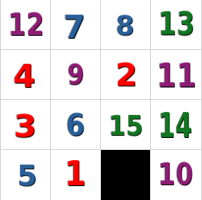
\includegraphics[width=0.25\linewidth]{chapter2/fig/puzzle.png}
	\caption{Example of a sliding puzzle}
	\label{fig:sliding_puzzle}
\end{figure}

\section{Conditions for solvability}
Even and odd sized boards are analysed separately (where size = N).

For odd sized boards where N is odd we have the puzzle only being solvable if and only if the boards
has an even number of inversions. The proof for this can be deduced by looking at Figure 2 and noting that for every switch of the blank block we have an even change in the sum of inversions of the board. \cite{princeton_8puzzle_assignment}

\begin{figure}[!htb]
	\centering
	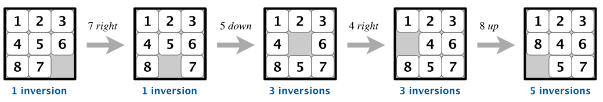
\includegraphics[width=1\linewidth]{chapter2/fig/princeton_odd_boards.png}
	\caption{Odd boards with change in blank piece only having even inversion change \cite{princeton_8puzzle_assignment}}
	\label{fig:sol_odd_board}
\end{figure}

For even sized boards where N is even we have the board solvable if and only if the number of
inversions plus the row of the blank square is odd. This is illustrated in Figure 3.

\begin{figure}[!htb]
	\centering
	\includegraphics[width=1\linewidth]{chapter2/fig/princeton_even_board_solvability.png}
	\caption{Even board solvability \cite{princeton_8puzzle_assignment}}
	\label{fig:sol_even_board}
\end{figure}

Half of all puzzle configurations are unsolvable. \cite{Notes_15_puzzle} This means that we only have N! / 2 configurations
that are solvable for an NxN board. This was proven using parity in the paper in \cite{Notes_15_puzzle}. Sliding puzzles
can be solved relatively quickly with today’s processing of computers for puzzles for example an 5x5
puzzle was solved in 205 tile moves in 2016. \cite{Domain_cube_forum}

The issue more so lies in finding the shortest path to solving a puzzle. This specific problem of solving
with the least amount of tile moves of a sliding puzzle has been defined as NP (non-deterministic polynomial-time) hard. NP hardness is are problems that are as least as hard as NP.
Where in computational complexity theory NP (non-deterministic polynomial-time) is a has a solution
with a proof variable to be in polynomial time by a deterministic Turing Machine. A Turing machine is
a mathematical model defining an abstract machine which manipulates symbols according to a set of
rules. \cite{Computation_finite_and_infinite_machines}

In simpler terms a problem is NP if it can be solved within a time that is a polynomial function of the
input. For instance if we define the time to solve a problem as ‘T’ and the input data as ‘D’. Then as
long as T = polynomial function (D) then a problem is NP.